\documentclass[12pt, a4paper]{article}                      % use "amsart" instead of "article" for AMSLaTeX format
\usepackage[a4paper,margin=1in]{geometry}                   % Adjust margins
\usepackage{amsmath,amssymb,listings,color,textcomp,adjustbox,tikz,pgfplots}        % Math packages: amsmath, amssymb, listings, color
\usepgfplotslibrary{external,fillbetween}
\pgfplotsset{compat=1.14}
\usepackage[makeroom]{cancel}
\title{\bf{Homework \textnumero 6}}
\author{Author: David Oniani
\\
\ \ \ Instructor: Tommy Occhipinti}
\date{October 07, 2018}

\usepackage{listings}
\usepackage{color}

\newcommand{\natn}{\mathbb{N}}
\newcommand{\intz}{\mathbb{Z}}
\newcommand{\intzp}{\mathbb{Z^+}}
\newcommand{\intzn}{\mathbb{Z^-}}

\definecolor{dkgreen}{rgb}{0,0.6,0}
\definecolor{gray}{rgb}{0.5,0.5,0.5}
\definecolor{mauve}{rgb}{0.58,0,0.82}
\definecolor{backcolour}{rgb}{0.95,0.95,0.92}

\lstset{
backgroundcolor=\color{backcolour},
aboveskip=3mm,
belowskip=3mm,
showstringspaces=false,
columns=flexible,
basicstyle={\small\ttfamily},
numbers=left,
numberstyle=\normalsize\color{gray},
keywordstyle=\color{blue},
commentstyle=\color{dkgreen},
stringstyle=\color{mauve},
breaklines=true,
breakatwhitespace=true,
tabsize=4
}


\begin{document}
\maketitle


\begin{itemize}
\item[36.]
Prove that if $S$ and $T$ are shifty sets (in the sense of a previous exercise) then $S \cup T$
is also a shifty set.
\begin{quote}
Let's first remember what it means to be shifty.
A subset $S$ of $\intz$ is called shifty if for every $x \in S$, $x - 1 \in S$ or $x + 1 \in S$.\\
Let's consider the following two cases:
\begin{itemize}
\item[1.]
Let $x \in S$ and prove that $x - 1$ or $x + 1$ is in $S \cup T$
\item[2.]
Let $y \in T$ and prove that $y - 1$ or $y + 1$ is in $S \cup T$
\\\\
Let's first consider the case when $x \in S$ and prove that $x - 1$ or $x + 1$ is in $S \cup T$.
If $x \in S$, since $S$ is shifty, it means that either $x - 1 \in S$ or $x + 1 \in S$. Union $S \cup T$
will have all the members of $S$ thus, it means that either $x - 1 \in S \cup T$ or $x + 1 \in S \cup T$.
\\\\
Now let's show that if $y \in T$, $y - 1$ or $y + 1$ is in $S \cup T$.
If $y \in T$, since $T$ is shifty, it means that either $y - 1 \in T$ or $y + 1 \in T$. Union $S \cup T$
will have all the members of $T$ thus, it means that either $y - 1 \in S \cup T$ or $y + 1 \in S \cup T$.
\\\\
Thus, we considered all the cases and proved that if $S$ and $T$ are shifty sets (in the sense of a previous exercise) then $S \cup T$
is also a shifty set.
\end{itemize}
\begin{flushright}
\textit{Q.E.D.}
\end{flushright}
\end{quote}

\item[37.]
Prove that $n \in \intz$ then $1 + (-1)^n(2n-1)$ is a multiple of 4.
\begin{quote}
Since $n \in \intz$, it is either even or odd. Let's consider two cases:
\begin{itemize}
\item[1.]
$n$ is even
\item[2.]
$n$ is odd
\end{itemize}

If $n$ is even, then $n = 2k$ where $k \in \intz$. We get:
$$1 + (-1)^n(2n-1) = 1 + (-1)^{2k}(2 \times 2k-1) = 1 + 4k - 1 = 4k \mbox{, where } k \in \intz$$
Hence, we got that if $n$ is even, $1 + (-1)^n(2n-1) = 4k$ where $k \in \intz$. Thus, if $n$ is even,
$1 + (-1)^n(2n-1)$ is a multiple of 4.

If $n$ is odd, then $n = 2k + 1$ where $k \in \intz$. We have:
$$1 + (-1)^n(2n-1) = 1 + (-1)^{2k+1}(2 \times (2k + 1)-1) = 1  - (4k + 2 - 1) = -4k \mbox{ where } k \in \intz$$
Thus, we got that if $n$ is odd, $1 + (-1)^n(2n-1) = -4k$ where $k \in \intz$. Hence, if $n$ is odd,
$1 + (-1)^n(2n-1) = -4k$ is a multiple of 4.
\\\\
Finally, since integers could either be odd or even, we considered all the cases ($n$ is even and $n$ is odd) and in
both of the cases, $1 + (-1)^n(2n-1)$ is a multiple of 4. Thus, if $n \in \intz$, $1 + (-1)^n(2n-1)$ is a multiple of 4.
\begin{flushright}
\textit{Q.E.D.}
\end{flushright}
\end{quote}

\item[38]
Prove that if $n \in \intzp$ is odd then $n^2 - 1$ is divisible by 8.
\begin{quote}
Suppose $n$ is odd. Then $n = 2k + 1$ where $k \in \intzp \cup \{0\}$.
Then we have:
$$n^2 - 1 = (2k + 1)^2 - 1 = 4k^2 + 4k + 1 - 1 = 4k^2 + 4k = 4k \times (k + 1)$$
Thus, if $n$ is odd, $n^2 - 1 = 4k \times (k + 1)$ where $k \in \intzp \cup \{0\}$.
Since $k$ is in the set of positive integers or equals 0, we can consider the following
three cases:
\begin{itemize}
\item[1.]
$k$ is 0
\item[2.]
$k$ is even
\item[3.]
$k$ is odd\\
\end{itemize}
If $k = 0$, $n^2 - 1 = 4k \times (k + 1) = 4 \times 0 \times (0 + 1) = 0$ which is divisible by 8.
\\\\
If $k$ is even, $k = 2l$ where $l \in \intzp$ (not including zero since we already considered that case above).
Then $n^2 - 1 = 4k \times (k + 1) = 8 \times (l \times (2l + 1))$ which is divisible by 8.
\\\\
If $k$ is even, $k = 2l + 1$ where $l \in \intzp$.
Then $n^2 - 1 = 4k \times (k + 1) = 4 \times (2l + 1) \times (2l + 2) = 8 \times ((2l + 1) \times (l + 1))$ which
is divisible by 8.
\\\\
Thus, we considered all the cases and we proved that if $n \in \intzp$ is odd then $n^2 - 1$ is divisible by 8.
\begin{flushright}
\textit{Q.E.D.}
\end{flushright}
\end{quote}

\item[39.]
Prove that every integer can be written as the sum of exactly 3 distinct integers. (For
example, $5 = 4 + 2 + (-1)$).
\begin{quote}
Suppose $k$ is an integer. Then, we should find three distinct integers such that they sum to $k$.
Now, let's consider the following integers:\\
$x = k + 1$, $y = -k - 1$, and $z = k$. It is clear that $x \neq z$ and $y \neq z$.\\
If $x = z$, we have $k + 1 = k \iff 1 = 0$ which is nonsensical.\\
If $y = z$, we have $-k - 1 = k \iff k = \dfrac{-1}{2}$ which is also
not possible because $k$ is an integer.\\
Thus $x \neq z$ and $y \neq z$, but we do not know if $x \neq y$.
Hence, we have to consider cases.
\\\\
Now, consider two cases:
\begin{itemize}
\item[1.]
$x \neq y$
\item[2.]
$x = y$
\end{itemize}
If $x \neq y$, we already know that $x \neq z$ and $y \neq z$ and thus we found three distinct integers which sum up to $k$, namely $x = k + 1$, $y = -k - 1$, and $z = k$.
\\\\
If $x = y$, we get $k + 1 = -k - 1$ and $k = -1$. However, even if $k = -1$, we can find three distinct integers, namely $x = -2$, $y = 2$, and $z = -1$.\\\\
Thus, we considered all the possible cases and we always find three integers which sum up to some random integer $k$.
Hence, every integer can be written as the sum of exactly 3 distinct integers.
\begin{flushright}
\textit{Q.E.D.}
\end{flushright}
\end{quote}
\item[40.]
Prove that if $x, y, \mbox{ and } z$ are integers then at least one of $x + y$, $x + z$, and $y + z$ is even.
\begin{quote}
Suppose, for the sake of contradiction, that $x + y$, $x + z$, and $y + z$ are all odd.\\\\
Now, without a loss of generality, consider the following four cases:
\begin{itemize}
\item[1.]
$x,y,z$ are all even
\item[2.]
$x,y,z$ are all odd
\item[3.]
$x,y$ are even and $z$ is odd
\item[4.]
$x,y$ are odd and $z$ is even
\end{itemize}
If $x,y,z$ are all even, $x = 2j$, $y = 2k$, $z = 2l$ where $j,k,l \in \intz$. Thus, we get:
$x + y = 2j + 2k = 2 \times (j + k)$ which is even.
\\\\
If $x,y,z$ are all odd, $x = 2j + 1$, $y = 2k + 1$, $z = 2l + 1$ where $j,k,l \in \intz$. Thus, we get:
$x + y = 2j + 1 + 2k + 1 = 2j + 2k + 2 = 2 \times (j + k + 1)$ which is even.
\\\\
If $x,y$ are even and $z$ is odd, $x = 2j$, $y = 2k$, $z = 2l + 1$ where $j,k,l \in \intz$. Thus, we get:
$x + y = 2j + 2k = 2 \times (j + k)$ which is even.
\\\\
If $x,y$ are odd and $z$ is even, $x = 2j + 1$, $y = 2k + 1$, $z = 2l$ where $j,k,l \in \intz$. Thus, we get:
$x + y = 2j + 1 + 2k + 1 = 2j + 2k + 2 = 2 \times (j + k) + 1$ which is even.
\\\\\\
Thus, we've considered all the possible cases and proved that if $x, y, \mbox{ and } z$ are integers then at
least one of $x + y$, $x + z$, and $y + z$ is even.
\begin{flushright}
\textit{Q.E.D.}
\end{flushright}
\end{quote}

\item[41.]
Prove or Disprove: There exist prime number $p$ and $q$ such that $p - q = 97$.
\begin{quote}
There are no prime numbers $p$ and $q$ such that $p - q = 97$. Let's prove it!
\\
First, notice that since $p$ and $q$ are prime, $p,q > 0$. Also, from $p - q = 97$,
we get $p = 97 + q$ and since $p,q > 0$, $p > q$. Thus, we have $0 < q  < p$.
Now, since $p - q$ is odd, it is the case that one of $p,q$ is odd and the other one is even
(because difference of even as well as odd numbers is even). However, we know that there is only
one even prime number, namely 2. Let's consider following two cases:
\begin{itemize}
\item[1.]
$p = 2$
\item[2.]
$q = 2$
\\
\end{itemize}
Since $0 < q < p$, we know that $p$ cannot be 2 (if $p = 2$,
there is no prime number below 2, so $q$ cannot be prime).
\\\\
If $q = 2$, $p - 2 = 97$ and $p = 99 = 3 \times 3 \times 11$ which is not prime.
\\\\
Thus, we considered all the cases and there are no prime numbers, $p$ and $q$,
of which the difference is 97.
\begin{flushright}
\textit{Q.E.D.}
\end{flushright}
\end{quote}
\item[42.]
For $n \in \intzp$, we define the $n^{th}$ triangular number to be $T_n := 1 + 2 + ... + n$.
Thus we have $T_1 = 1, T_2 = 3, T_3 = 6, T_4 = 10, T_5 = 15$, and so on. We will prove later
that $T_n = \dfrac{n(n+1)}{2}$, and you should use that formula for this problem. Prove that
for $n \in \intzp$, $T_n$ is odd if and only if $n$ is 1 or 2 more than a multiple of $4$.
\begin{quote}
Since it is the "if and only if" proof, let's split the proof in two cases:
\begin{itemize}
\item[1.]
Prove that if $n$ is 1 or 2 more than a multiple of 4, $T_n$ is odd.
\item[2.]
Prove that if $n$ is not 1 and is not 2 more than a multiple of 4, $T_n$ is not odd (thus is even).
\end{itemize}
\textbf{Let's first prove that if $n$ is 1 or 2 more than a multiple of 4, $T_n$ is odd.}\\\\
If $n$ is 1 more than a multiple of 4, $n = 4k + 1$ where $k \in \intzp$. Then we have:
$$T_n = \dfrac{n(n+1)}{2} = \dfrac{(4k + 1)((4k + 1) + 1)}{2} = \dfrac{(4k + 1)(4k + 2)}{2} = (4k + 1) \times (2k + 1).$$
Thus, we have that if $n$ is 1 more than a multiple of 4, $T_n = (4k + 1) \times (2k + 1)$, where $k \in \intzp$, which is a multiplication of two
odd numbers and thus is odd.
\\\\
If $n$ is 2 more than a multiple of 4, $n = 4k + 2$ where $k \in \intzp$. Then we have:
$$T_n = \dfrac{n(n+1)}{2} = \dfrac{(4k + 2)((4k + 2) + 1)}{2} = \dfrac{(4k + 2)(4k + 3)}{2} = (2k + 1) \times (4k + 3)$$
Hence, we got that $T_n = (2k + 1) \times (4k + 1) = (2k + 1) \times (4k + 3)$ which the multiplication of two odd
numbers and thus, if $n$ is 2 more than a multiple of 4, $T_n$ is odd.
\\\\
\textbf{Now, let's prove that if $n$ is not 1 or 2 more than a multiple of 4, $T_n$ is even.}\\\\
If $n$ is not $1$ and is not two more than a multiple of four, we have the following five cases to consider:
\begin{itemize}
\item[1.]
$n = 4k$ where $k \in \intzp$
\item[2.]
$n = 4k + 3$ where $k \in \intzp$
\end{itemize}
If $n = 4k$ where $k \in \intzp$, $T_n = \dfrac{4k(4k+1)}{2} = 2 \times (k(4k + 1))$ which is even.
\\\\
If $n = 4k + 3$ where $k \in \intzp$, $T_n = \dfrac{(4k+3)(4k+4)}{2} = 2 \times ((4k + 3)(2k + 2))$ which is even.
\\\\
NOTE: SINCE WE CONSIDERED INTEGERS STARTING AT 4 (SINCE WE ASSUMED THAT $n = 4k,4k+1,4k+2,4k+3$ where $k \in \intzp$,
the smallest number we get is $n = 4 \times 1 = 4$), NOW WE NEED TO CHECK $T_n$ for 1,2, and 3.
\\\\
If $n = 1$, $T_n = \dfrac{1(1+1)}{2} = 1$ which is odd and indeed, 1 = 0 + 1 and 0 is a multiple of 4 (thus, 3 has $4l + 1$ form where $l \in \intz$)..
\\
If $n = 2$, $T_n = \dfrac{2(2+1)}{2} = 3$ which is odd and indeed, 2 = 0 + 2 and 0 is a multiple of 4 (thus, 3 has $4l + 2$ form where $l \in \intz$)..
\\
If $n = 3$, $T_n = \dfrac{3(3+1)}{2} = 6$ which is even and indeed, 3 = 0 + 3 and 0 is a multiple of 4 (thus, 3 has $4l + 3$ form where $l \in \intz$).
\\\\
Thus, we considered all the cases and proved that for $n \in \intzp$, $T_n$ is odd if and only if $n$ is 1 or 2 more
than a multiple of $4$.
\begin{flushright}
\textit{Q.E.D.}
\end{flushright}
\end{quote}
\newpage
{\large Bookwork}
\item[2.]
Solve the equality $|x + 1| < |x^2 - 1|$. Interpret results geometrically.
\begin{quote}
Let's consider the following two cases:\\
\begin{itemize}
\item[1.]
$x + 1 \geq 0$
\item[2.]
$x - 1 \leq 0$
\\
\end{itemize}

\textbf{Let's first consider the case} $x + 1 \geq 0$.\\
If $x + 1 \geq 0$, the inequality will have a form:
$$x + 1 < |x^2 - 1|$$
Now, let's consider another two cases:
\begin{itemize}
\item[1.]
$x^2 - 1 \geq 0$
\item[2.]
$x^2 - 1 \leq 0$
\\
\end{itemize}
If $x^2 - 1 \geq 0$, the equality we get is:\\
$$x + 1 < x^2 - 1$$
And we get:
$$x^2 - x - 2 > 0$$
And finally, $x \in (-\infty, -1) \cup (2, +\infty)$.\\
But since $x + 1 \geq 0$, $x \geq -1$ and we get $x \in (2, +\infty)$
\\\\\\
If $x^2 - 1 \leq 0$, the equality we get is:\\
$$x + 1 < -x^2 + 1$$
And we get:
$$x^2 + x < 0$$
And finally, $x \in (-1, 0)$.\\
It also satisfies $x + 1 \geq 0$.
\\\\\\
\textbf{Now, let's consider the second case,} $x + 1 \leq 0$.\\
If $x + 1 \leq 0$, the inequality will have a form:
$$-x - 1 < |x^2 - 1|$$
Now, as previously, let's consider another two cases:
\begin{itemize}
\item[1.]
$x^2 - 1 \geq 0$
\item[2.]
$x^2 - 1 \leq 0$
\\
\end{itemize}
If $x^2 - 1 \geq 0$, the equality we get is:\\
$$-x - 1 < x^2 - 1$$
And we get:
$$x^2 + x > 0$$
And finally, $x \in (-\infty, -1) \cup (0, +\infty)$.\\
But since $x + 1 \leq 0$, $x \leq -1$ and we get $x \in (-\infty, -1)$
\\\\\\
If $x^2 - 1 \leq 0$, the equality we get is:\\
$$-x - 1 < -x^2 + 1$$
And we get:
$$x^2 - x -2 < 0$$
And finally, $x \in (-1, 2)$.\\
But since $x + 1 \leq 0$, $x \leq -1$ and we do not get any solutions for this inequality.
\\\\
Thus, we got the following answers: $x \in (2, +\infty)$, $x \in (-1, 0)$, $x \in (-\infty, -1)$.\\
Finally, by merging these answers, we get: $x \in (-\infty, -1) \cup (-1,0) \cup (2, +\infty)$.

\begin{center}
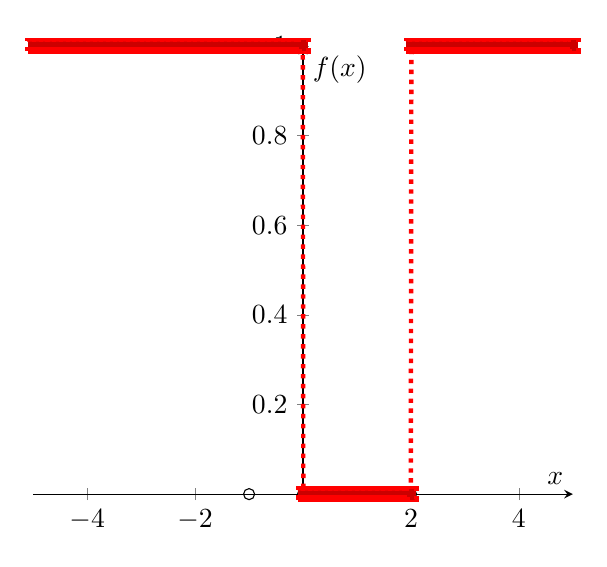
\begin{tikzpicture}
\begin{axis}[
axis lines=center,
xlabel=\(x\),
ylabel=\(f(x)\),
restrict y to domain=-50:50,
samples=1000,
]

\addplot [only marks, mark=o] table {
-1 0
0 0
2 0
};
\def\ymin{\pgfkeysvalueof{/pgfplots/ymin}}
\def\ymax{\pgfkeysvalueof{/pgfplots/ymax}}
\addplot+[style=dotted, style=ultra thick] {abs(x+1) < abs(x^2 - 1)};

\end{axis}
\end{tikzpicture}
\end{center}
This line shows that $x \in (-\infty, -1) \cup (-1,0) \cup (2, +\infty)$.
Part where $x \in (0,2)$ is in between two horizontal dotted lines meaning that
it is not the part of the solution. Also, $x = -1$ is also not in the set (you can see a little circle
there which basically means that the point is out and $x \neq -1$).
\end{quote}

\item[4.]
\begin{itemize}
\item[(a)]
\item[]
Show that any integer can be written in the form $10q + r$ where $0 \leq r \leq 9$.
\begin{quote}
I don't really like the way this is phrased, so I will rephrase what we have to prove.
We have to prove that:\\
\begin{center}
for every integer $k$, there exists $q$ and $r$ such that $k = 10q + r$ and $0 \leq r \leq 9$.\\\
\end{center}
Notice that if an integer ends on 0, it is always divisible by 10. Thus, it is just the problem
of picking $r$ so that $k - r$ ends on 0 (if $k - r$ ends on zero we devide the result by 10 and get $q$).\\
Let's consider the following 10 cases for the possible endings of the number.
\begin{itemize}
\item
Number ends on 0
\item
Number ends on 1
\item
Number ends on 2
\item
Number ends on 3
\item
Number ends on 4
\item
Number ends on 5
\item
Number ends on 6
\item
Number ends on 7
\item
Number ends on 8
\item
Number ends on 9
\\
\end{itemize}
\begin{itemize}
\item
If number ends on 0, we can pick $r = 0$, and then $k$ is divisble by 10 and we get the value of $q$.\\
\item
If number ends on 1, we can pick $r = 1$, and then $k$ is divisble by 10 and we get the value of $q$.\\
\item
If number ends on 2, we can pick $r = 2$, and then $k$ is divisble by 10 and we get the value of $q$.\\
\item
If number ends on 3, we can pick $r = 3$, and then $k$ is divisble by 10 and we get the value of $q$.\\
\item
If number ends on 4, we can pick $r = 4$, and then $k$ is divisble by 10 and we get the value of $q$.\\
\item
If number ends on 5, we can pick $r = 5$, and then $k$ is divisble by 10 and we get the value of $q$.\\
\item
If number ends on 6, we can pick $r = 6$, and then $k$ is divisble by 10 and we get the value of $q$.\\
\item
If number ends on 7, we can pick $r = 7$, and then $k$ is divisble by 10 and we get the value of $q$.\\
\item
If number ends on 8, we can pick $r = 8$, and then $k$ is divisble by 10 and we get the value of $q$.\\
\item
If number ends on 9, we can pick $r = 9$, and then $k$ is divisble by 10 and we get the value of $q$.\\
\end{itemize}
Thus, we considered all the possible cases and proved that any integer can be written in the form $10q + r$ where $0 \leq r \leq 9$.
\begin{flushright}
\textit{Q.E.D.}
\end{flushright}
\end{quote}
\item[(b)]
\item[]
Show that the square of any integer ends in 0, 1, 4, 5, 6, or 9.
\begin{quote}
There are 9 numbers on which an integer could end.\\
These numbers are: 0, 1, 2, 3, 4, 5, 6, 7, 8, 9.\\
Then let's consider the following 10 cases.
\begin{itemize}
\item
Number ends on 0
\item
Number ends on 1
\item
Number ends on 2
\item
Number ends on 3
\item
Number ends on 4
\item
Number ends on 5
\item
Number ends on 6
\item
Number ends on 7
\item
Number ends on 8
\item
Number ends on 9
\end{itemize}
If number ends on 0, its square ends on the same number as $0^2$ ends on, thus on 0.\\
If number ends on 0, its square ends on the same number as $1^2$ ends on, thus on 1.\\
If number ends on 0, its square ends on the same number as $2^2$ ends on, thus on 4.\\
If number ends on 0, its square ends on the same number as $3^2$ ends on, thus on 9.\\
If number ends on 0, its square ends on the same number as $4^2$ ends on, thus on 6.\\
If number ends on 0, its square ends on the same number as $5^2$ ends on, thus on 5.\\
If number ends on 0, its square ends on the same number as $6^2$ ends on, thus on 6.\\
If number ends on 0, its square ends on the same number as $7^2$ ends on, thus on 9.\\
If number ends on 0, its square ends on the same number as $8^2$ ends on, thus on 4.\\
If number ends on 0, its square ends on the same number as $9^2$ ends on, thus on 1.\\
\\
Thus, the ending numbers we got are: 0, 1, 4, 9, 6, 5, 6, 9, 4, 1.\\
Now, if we eliminate the duplicates, we get: 0, 1, 4, 5, 6, and 9.
\begin{flushright}
\textit{Q.E.D.}
\end{flushright}
\end{quote}
\end{itemize}
\item[8.]
Can one form a ten-digit integer by putting a digit between 0 and 9 in the empty
boxes in the given table as follows: The digit in the box labeled 0 indicates the
number of times 0 appears in the number, the digit in box 1 indicated the number
of times 1 appears in the number, etc.?
\begin{table}[h!]
	\centering
	\begin{adjustbox}{max width=\textwidth}
	\resizebox{0.6\linewidth}{!}
	{
		\begin{tabular}{*{10}{|c}|}
		\hline
		0 & 1 & 2 & 3 & 4 & 5 & 6 & 7 & 8 & 9\\ \hline
		  &   &   &   &   &   &   &   &   & \\
        \hline
	\end{tabular}
    }
	\end{adjustbox}
\end{table}
\\
(For instance, if 9 is placed in box 0, then the remaining boxes must be filled with
0 in order that the nine zeros actually appear. In this case, however, we reach a contradiction
since box 9 cannot contain 0 as at least one 9 appears in the number. Thus the desired ten-digit
number cannot have 9 as its leftmost digit.)(Hint: Consider the possible ways of filling the box
labeled 0.) How many such numbers exist?
\begin{quote}
\begin{itemize}
\item[**]
If 9 is placed in box 0, we reach the contradiction since box 9 cannot cointain 0 as at least one 0 appears in the number.
\item[**]
If 8 is placed in box 0, we have eight 0s and 8 itself in the number, then we are left with only one box. Notice that since 8 is under
the box labeled 0, we should have 1 under box labeled 8, but then we should also have 1s but we are out of boxes. Thusm, we
reach the contradiction that there is no way to have 8 zeros. 
\item[**]
If 7 is placed in box 0, it means that we must have seven 0s and 7 itself in the number, then we are left with 2 boxes. Now, since 7 is
under box labeled 0, there must be 1 under box labeled 7. But then we should also have 1 under box labeled 1. However, now we have two 1s
and we said that there is only one and we are even out of boxes. Hence, we reach the contradiction.
\item[**]
If 6 is placed under the box 0, box 6 should be 1 . Then we should have at least one 1.
However, now we have two 1s, thus box labeled 2 must be 1 and box labeled 1 must be two and we are actually left with six 0s (ALL BOXES ARE FILLED WITH NUMBERS).
And we got a number! It's 6210001000. It has ten digits, six 0s, two 1s, one 2, zero 3s, zero 4s, zero 5s, one 6s, zero 7s, zero 8s, zero 9s.
\item[**]
If 5 is placed under the box 0, box 5 should be 1 and we are left with 3 empty boxes. Now, if we have one 1, box under label 1 should also be 1.
Now, we have two 1s, so box under label one should be 2 and the box under label 2 should be 1. But if we do these operations, we will actually have
six 0s while we need to have 5 and will end up with 5210010000. Thus, we reach the contradiction.
\item[**]
If 4 is placed under the box 0, with the same reasoning, we end up with 4210100000 but then we have six 0s and we reach the contradiction.
\item[**]
If 3 is placed under the box 0, with the same reasoning, we end up with 3211000000 but then we have six 0s while we need 3 and we reach the contradiction.
Thus, we reach the contradiction.
\item[**]
If 2 is placed under the box 0, we have to write 1 under the box 2, but now we have one 1 as well hence, we have
to write 2 under box labeled 2 and with the same reasoning as above, we cannot fill in all of these numbers.
Thus, we reach the contradiction.
\item[**]
Case when 1 is placed under the box labeled 0 is also not possible. If we place 1 under box labeled 0, it means that the number has one 0 and we have to put
1 under box labeled 1. Then we end up with 1100000000 which is seven 0s when we need only 1 and we reach the contradiction.
\item[**]
If 0 is placed under the label 0, it means that at least one number occurs twice, but then
it means that we will end up with 11 digits in the end.
\\
\end{itemize}
Thus, we can construct a ten-digit number with this approach. The number is 6210001000.
And there is only one number like this (6210001000). Hence, the answer is yes and there
is only one such number which is 6210001000.
\end{quote}
\end{itemize}
\end{document}
